This paper describes the replication of the computational model of the `\emph{two-pathways to the amygdala}'~\supercite{Ledoux1992,Romanski1992}, as well as the classical conditioning experiment originally implemented by~\citet{Armony1995}. The original article had two main objectives. As with any other research project, the main goal was to validate a set of `\emph{principles}' on which the computational model was built, and verify that those principles could account for a set of physiological and behavioral results from classical conditioning studies. However, hidden behind this first standard aim was the desire to highlight the usefulness of computational models in helping neuroscience move forward. By their very nature computational models are the perfect tool to validate the mechanisms that brain systems are theorized to implement. Furthermore, once the validity of a computational model has been established it can serve as an abstract stand-in for the animal's brain. Hence, allowing researchers to easily perform lesion studies and make predictions that can later be more efficiently validated by neuroscience~\supercite{Armony1997,Armony1997a}. Effectively, this establishes a feedback loop between computational models and neuroscience.\\

The sections making up this paper have been organized to mirror the layout of the original article~\supercite{Armony1995}. As such, the first section introduces the model of the two pathways to the amygdala as suggested by~\citet{Ledoux1992}, before describing the neural structure implemented by~\citet{Armony1995} to validate said model. The next section details the fear conditioning experiment used as a testing ground. Both of those sections also address the various issues encountered while reproducing the original simulation. The third section presents the results gathered by re-implementing both the neural network and classical conditioning experiment. Finally, the last section concludes by discussing the differences between the results published by~\citet{Armony1995} and those collected in this replication.

\section{A neural network constrained by fear}\label{sec:armonyModel}
As stated above, the main goal of~\citet{Armony1995} was to test the ability of three principles to explain two sets of behavioral and physiological findings. To do so,~\citet{Armony1995} designed and implemented a neural structure based on the following assumptions:
\begin{enumerate}
   \item Processing units: populations of real cells coding for the same piece of information can be abstracted as non-linear summing devices;
   \item Dual pathway connectivity: sensory information describing the state of the environment is encoded by two parallel systems, before converging on the amygdala;
   \item Learning: the synaptic strength for the connections between neurons is updated using a modified Hebbian learning rule, also known as the Stent-Hebb rule~\supercite{stent_physiological_1973}.
\end{enumerate}
Simulating a fear conditioning experiment,~\citet{Armony1995} explored whether the neural network would express conditioned responses similar to those observed in animals and known to be the result of amygdala activation. At the physiological level,~\citet{Armony1995} examined if the neural units displayed any change in activities as a result of conditioning analogous to those measured in single-cell recordings.

\subsection{Two pathways to the amygdala}
Based on a set of fear conditioning experiments and lesion studies, involving the `\emph{medial geniculate body}' (MGB), an area of the thalamus responsible for the transmission of data related to sound, as well as the auditory cortex~\citet{Ledoux1992} was able to conclude that stimuli entering the brain are forwarded to the amygdala following two parallel pathways. The first pathway projects directly from the medial division of the MGB (MGm) to the amygdala, and carries unrefined representations of the Conditioned Stimulus (CS). The second pathway originates in the ventral division of the MGB (MGv) and targets the auditory cortex, which produces a more elaborate representation of the CS\@. Finally, the auditory cortex sends its output to the amygdala.\\

In the case where the CS is a simple tone, for example,~\citet{Romanski1992} determined that both pathways are functionally equivalent, even if the direct thalamo-amygdala pathway is faster than the thalamo-cortico-amygdala pathway. However, in more complex cases where the animal is conditioned to a tone of a specific frequency, using the thalamo-amygdala pathway alone the animal is incapable of differentiating between the CS and tones with contiguous frequencies, and reacts similarly to for all of them. Therefore, the indirect pathway through the cortex while slower provides more detailed information concerning the CS\@. This allows animals to discriminate between tones of adjacent frequencies~\supercite{Romanski1992} and react to the specific CS only.

\begin{figure}[!htbp]
\centering
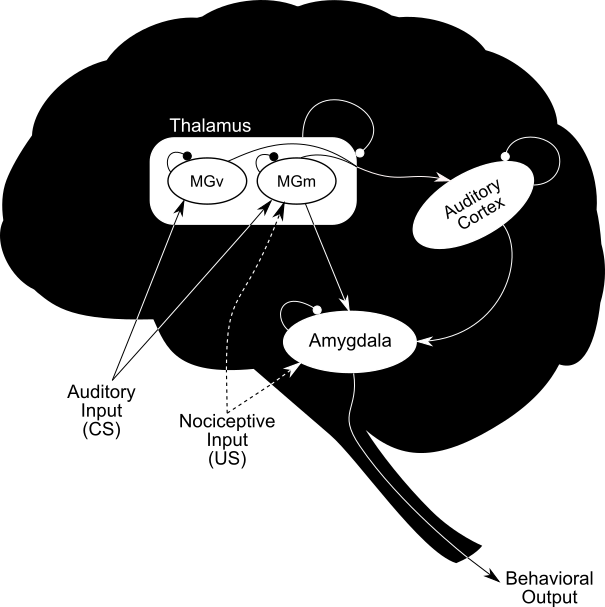
\includegraphics[width=0.65\textwidth]{Figs/armony}
\caption{\textit{Using the architecture depicted in this figure,~\citet{Armony1995} sought to validate the model of the `\emph{two-pathways to the amygdala}' suggested earlier by~\citet{Ledoux1992}. According to this model, sensory information entering the thalamus and destined for the amygdala takes two parallel paths. The first one links directly to the amygdala and provides fast communication, but at the cost of precision. The second path goes through the auditory cortex and further refines the signal, hence, providing much more detailed information to the amygdala. Therefore, the overall role of the first pathway is to ready the body for a `\emph{fight-or-flight}' response, while the second one helps decide if a reaction is actually necessary.}}\label{fig:armony}
\end{figure}

\subsection{Model}
The model suggested by~\citet{Armony1995} is split into two modules, each corresponding to one of the pathways to the amygdala. As shown in Figure~\ref{fig:armony}, the first module includes the medial section of the MGB (MGm) and a layer representing the amygdala. While the second module is made of the ventral section of the MGB (MGv) and the cortex, which receives data from both MGm and MGv, and then projects to the amygdala. Every layer is populated with non-linear processing units, whose activation value can be thought of as the average neural activity of a small population of real neurons coding for the same patterns. The processing units used for this model strike a balance between capturing the basic features of the response of a real cell and being computationally tractable. For each unit, its output remains null as long as its net input is below the threshold $x_{thr} = 0$, and it saturates upon reaching the cell's maximum firing rate, $x_{sat} = 1$:
\begin{equation}
   act(x) = 
   \begin{cases}
      0 & \quad \text{if } x - x_{thr} < 0 \\
      x - x_{thr} & \quad \text{if } 0 < x - x_{thr} < x_{sat} \\
      x_{sat} & \quad \text{if } x_{sat} < x - x_{thr}
   \end{cases}
\end{equation}

%% Connectivity
Where, in Figure~\ref{fig:armony}, one layer projects to another the author chose to fully connect every sending units to each of the receiving units. Therefore, the net input of any neuron is computed as the weighted sum of its sending units' activation values:
\begin{equation}
   net_{r} = \sum_{s} a_{s} \times \omega_{rs}
\end{equation}
Where $\omega_{rs}$ is the synaptic weight between the sending unit $s$ and the current receiving unit $r$.\\

%% Lateral inhibition
To account for the presence of inter-neurons in real brains, lateral inhibition has been implemented through a soft version of the winner-takes-all mechanism. Following this algorithm in each layer the winning unit (defined by strength of activation) inhibits all other units by an amount proportional to its net input: 
\begin{equation}
\begin{split}
   a_{win} &= activ(net_{win}) \quad \text{for the winner}\\ 
   a_{r} &= activ(net_{r} - \mu \times a_{win}) \quad \text{for the other units}
\end{split}
\end{equation}
$\mu$ was set to $0.2$ for all units, in all layers, and left unchanged for the whole duration of the experiment.\\

Within the original paper, the number of neural units per layer is only mentioned in the figure depicting the architecture, but nowhere are those quantities confirmed inside the text. However,~\citet{Armony1995} did bring up to the reader's attention the fact that in the competitive-learning scheme used for this model the number of input patterns for which a given unit is activated is inversely proportional to the number of units in the layer. Therefore, to capture the broad tuning capabilities of the first module, the MGm and amygdala layers have very few neurons. On the contrary, the MGv and cortical layers, both part of the second module are highly populated. Hence, allowing units in those groups to acquire a narrower tuning which accounts for the improved categorization capabilities of the cortex. Since we were unable to contact any of the original authors to ask for specific values regarding the size of each layer, we validated through trial and error that both the MGm and amygdala have $n = 3$ neural units, while the amount of neurons included in the MGv and cortical layers are more than double that, with $n=8$ for each.\\

%% Learning
After the presentation of each input pattern, learning is achieved through the modification of the synaptic weights of all excitatory connections. To update the weights~\citet{Armony1995} used a variant of the Hebbian learning rule, since it is well known that the direct application of Hebb's learning rule quickly leads to saturation. Therefore, to work around this issue, the so called Stent-Hebb algorithm was applied~\supercite{stent_physiological_1973}. It allows for both increases and decreases in synaptic strength based on the correlation in activity between the sending and receiving units. The equation used for updating the weights is:
\begin{equation}\label{equ:hebb1}
   \omega^{\prime}_{rs} = 
   \begin{cases}
      \omega_{rs} + \epsilon \times a_{r} a_{s} & \quad \text{if } a_{s} > a_{avg}\\
      \omega_{rs} & \quad \text{otherwise}
   \end{cases}
\end{equation}
Where $a_{avg}$ is the average activation value sampled over the units of the sending layer and $\epsilon = 0.1$ is the learning rate. Furthermore, to account for the decrease in synaptic strength for uncorrelated sending units, for each unit in the receiving layer the sum of its input weights is kept constant through multiplicative normalization. That is, each weight is further processed using the formula:
\begin{equation}\label{equ:normal}
   \omega_{rs} = \frac{\omega^{\prime}_{rs}}{\sum_{s} \omega^{\prime}_{rs}}
\end{equation}
As a consequence, the synaptic strength of sending units whose activation value remain below the layer's average will decrease, while the weights of correlated units increase.\\

In the simulated conditioning experiment, sound was used as the CS, while the nociceptive unconditioned stimulus (US) was represented by a single binary unit connected to all units within the MGm and amygdala layers (as depicted in Figure~\ref{fig:armony}). The strength of the synaptic connections between the US unit and the receiving neurons of the first module were set to $0.4$ and remained unchanged for the duration of the simulation. According to~\citet{Armony1995} this design decision was intended to ``\emph{capture the effect of diffuse somatosensory information associated with a US such as a footshock}''. A set of training patterns was created by dividing the auditory spectrum into $15$ pure tones of contiguous frequencies in an arbitrary scale. Consequently, the tones as well as the CS were represented in the simulation by overlapping patterns of activation in the input layer (as shown in Figure~\ref{fig:armony_input_feats}). In addition to the competitive learning algorithm (described in Equation~\ref{equ:hebb1} and Equation~\ref{equ:normal}), the use of overlapping nonorthogonal patterns facilitates the development of topographical representations of the input in the model's layers.\\

\begin{figure}[!htbp]
   \begin{center}
      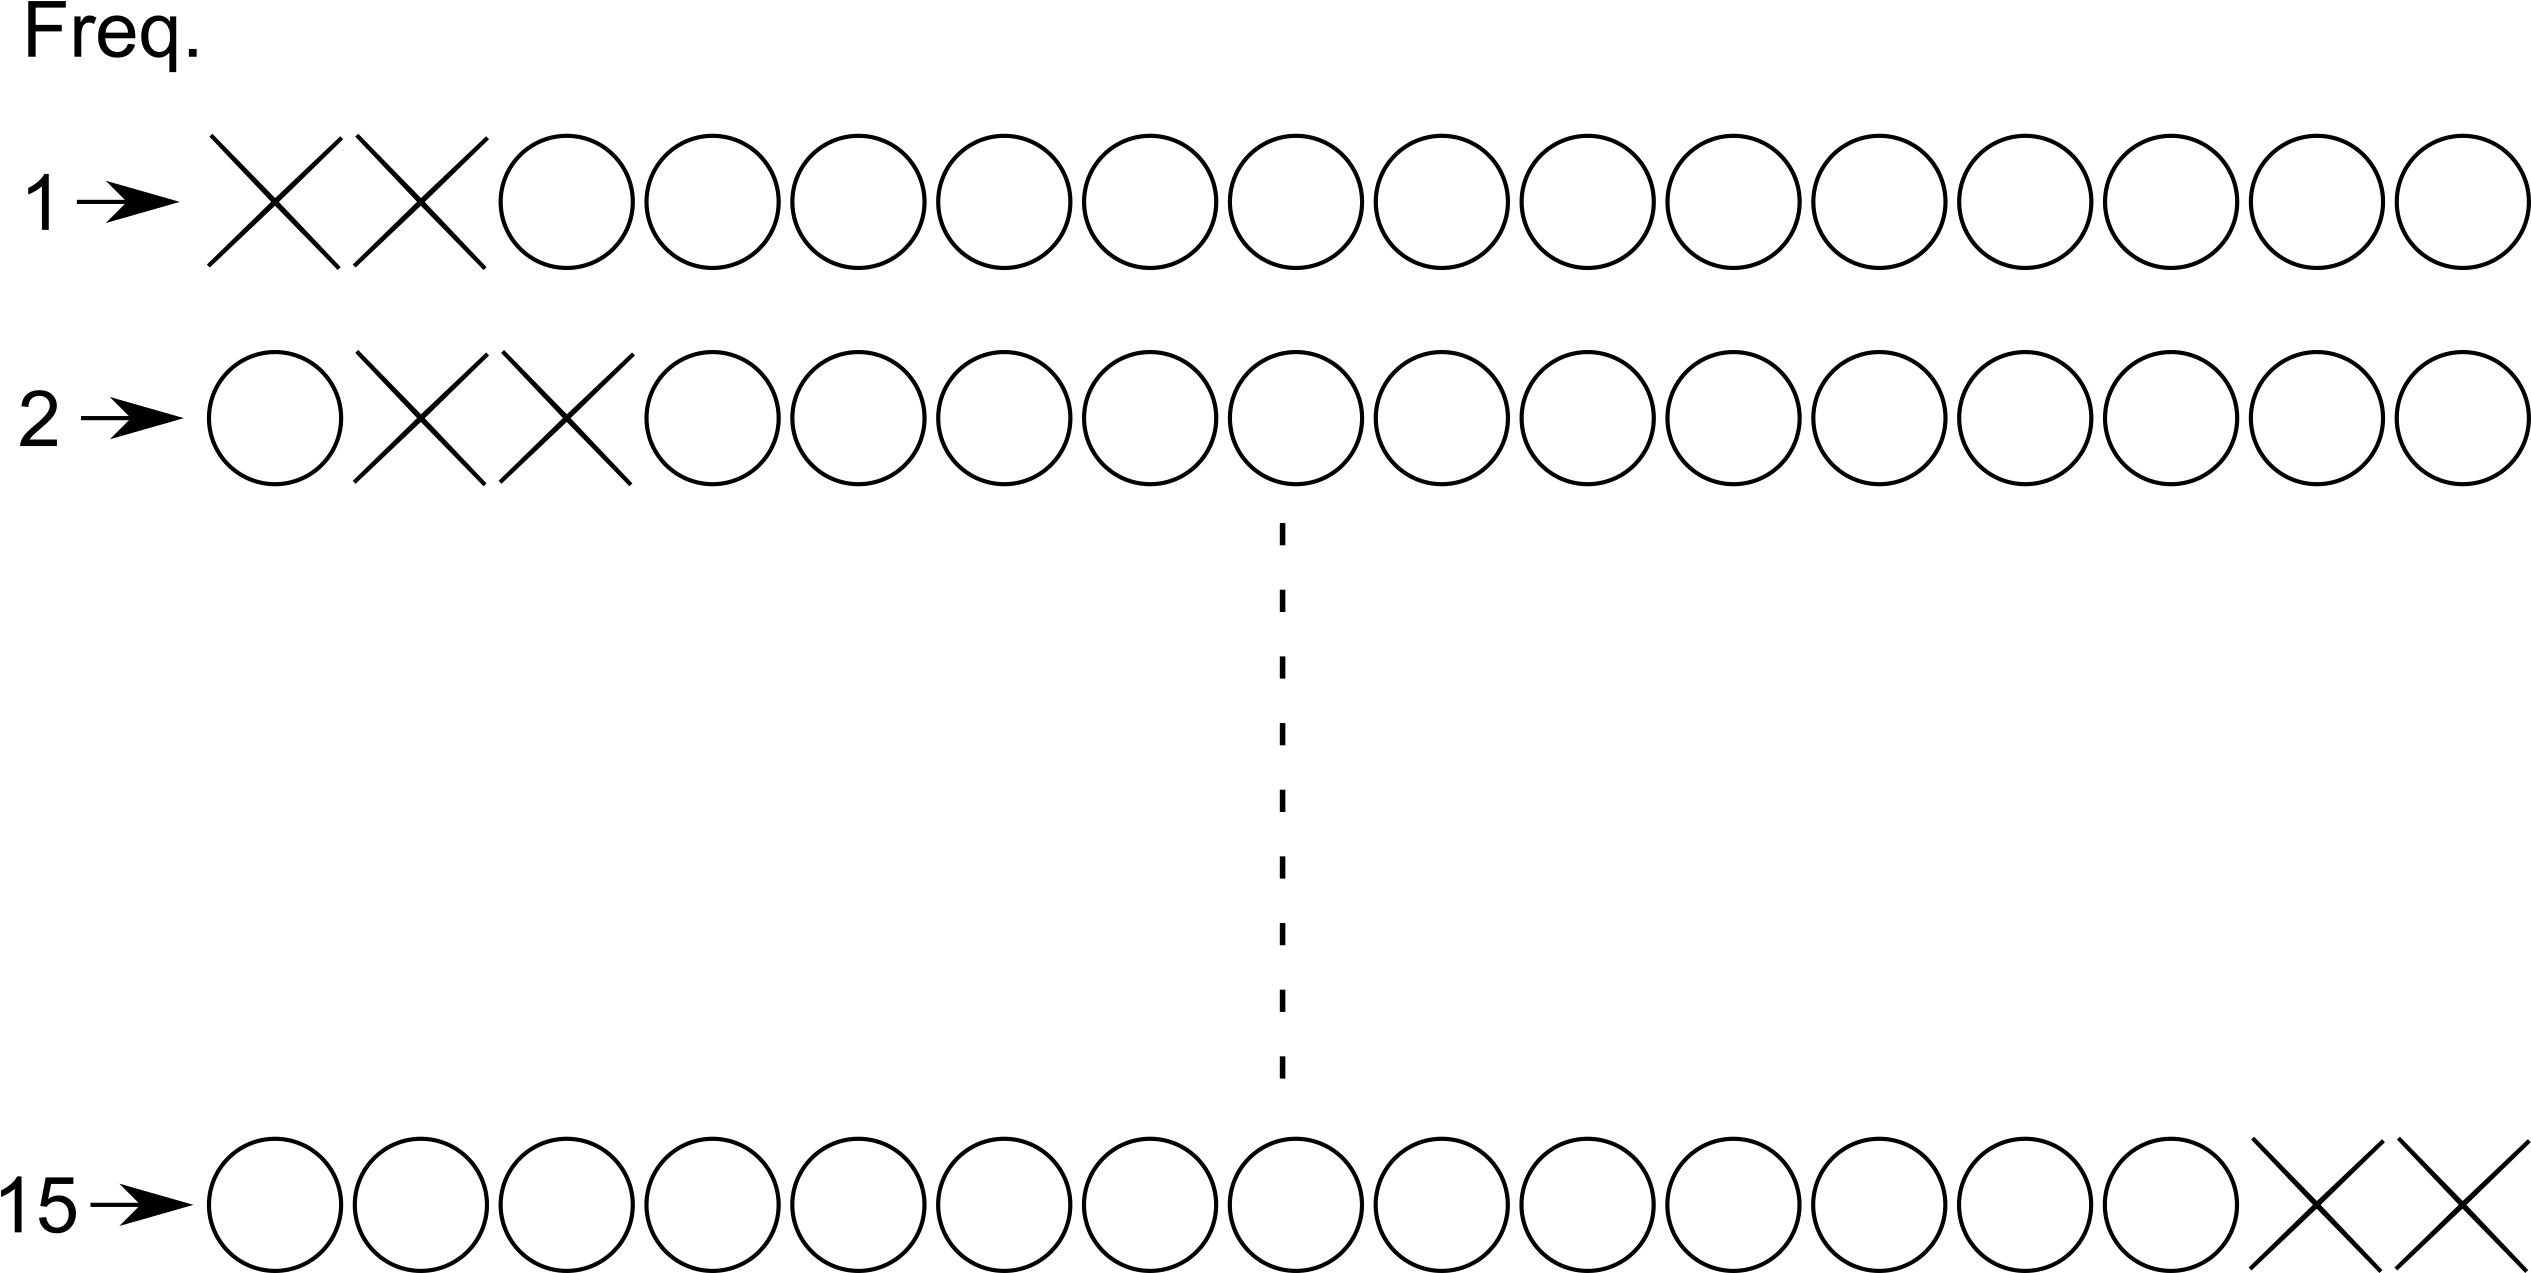
\includegraphics[width=0.6\textwidth]{Figs/input_features}
      \caption{\textit{This figure depicts the input features used in~\citeauthor{Armony1995}'s~\citeyearpar{Armony1995} conditioning experiment. Frequencies are represented by nonorthogonal overlapping patterns of activities in the input layer. When associated with the competitive learning mechanism (described in Equation~\ref{equ:hebb1} and Equation~\ref{equ:normal}), this type of pattern facilitates the development of topographical representations in the model's layers.}}\label{fig:armony_input_feats}
   \end{center}
\end{figure}

\section{Method}
As alluded to at the beginning of Section~\ref{sec:armonyModel}, to ascertain the validity of the model of the dual pathways to the amygdala suggested by~\citet{Ledoux1992},~\citet{Armony1995} simulated a fear conditioning experiment. The goal was to examine whether the neural network, whose implementation was guided by the principles expressed in Section~\ref{sec:armonyModel}, could reproduce the two sets of behavioral and physiological findings. At the behavioral level, it is expected that the network's behavioral output, defined as the sum total activity of the amygdala layer, should drastically increase for the frequency corresponding to the CS, while showing a net decrease in activity for all other frequencies. At the physiological level, the neural units within layers receiving information about the US, either directly or indirectly, are anticipated to have their receptive fields (RF) shift towards the CS's frequency. A neuron's receptive field is defined in this context as the frequency range for which its output activity is non-zero. The effects of conditioning should also be stronger the closer a unit's best frequency (BF\@; the frequency for which a neuron is maximally activated) was to the CS in the pre-conditioning phase. The fear conditioning experiment has been split into three distinct phases.\\

%% Development
Rather than programmatically constrain the initial synaptic weights so that input patterns would be represented topographically in all layers,~\citet{Armony1995} decided to randomly initialize the synaptic strengths with values in the range $[0, 1]$, then let the learning algorithm do the synaptic pruning. According to~\citet{Armony1995}, this is to ensure that any modification in the receptive fields of the neural units is the result of conditioning alone, and not an unforeseen consequence of setting a specific set of weights. Consequently, the first, `\emph{development}', phase consists in presenting sequentially all input patterns to the network without activating the nociceptive US unit. After each pattern, the weights of the excitatory connections were updated using the Stent-Hebb rule described in Equation~\ref{equ:hebb1}, and normalized unit-wise using Equation~\ref{equ:normal}. The loop was repeated until all units within the neural network had developed a stable RF\@. The curves labeled `\emph{Pre}' in Figures~\ref{fig:armony_act_mgm} ---~\ref{fig:armony_act_amyg}, show standard receptive fields for units belonging to each layers.\\

%% Conditioning
Once all units in the neural network had developed stable topographic representations for all input patterns, the conditioning paradigm was simulated. The `\emph{conditioning}' phase is very similar to the previous development phase. The only difference is that, a frequency was arbitrarily chosen to be the CS, and, therefore, associated with the activation of the nociceptive US unit. All input patterns were again sequentially presented to the input layers. The weights of the excitatory connections were adjusted following the same extended Stent-Hebb rule (defined in Equation~\ref{equ:hebb1} and Equation~\ref{equ:normal}). Again, the process repeated until the RFs of all units stabilized. The curves labeled `\emph{Post}' in Figures~\ref{fig:armony_act_mgm} ---~\ref{fig:armony_act_amyg} depict the new receptive fields units developed as a result of conditioning.\\

%% Testing
Finally, the `\emph{testing}' phase spreads across both of the previous phases. By measuring the sum total response of the amygdala's units (the behavioral response),~\citet{Armony1995} investigated the overall behavior of the network in response to the CS before and after conditioning (see Figure~\ref{fig:armony_behav_resp}). Additionally, for all neural units in the network their activation values for each of the frequencies  were also recorded after the first two phases to analyze any change in receptive fields between pre- and post-conditioning (shown in Figures~\ref{fig:armony_act_mgm} ---~\ref{fig:armony_act_amyg}).

\section{Results}
The present section analyzes the results we gathered by re-implementing both the computational model and classical conditioning experiment described so far using the Python language. The consistency of the replicated results with those published in the original paper~\supercite{Armony1995} is discussed in the next section, which concludes this article.\\

At the beginning of the development phase, when the synaptic strengths were randomly initialized neurons responded, on average, equally but weakly to all input patterns. By repeatedly presenting the $15$ tones to the network's inputs and adapting the weights of the excitatory connections using the competitive algorithm defined in Equation~\ref{equ:hebb1} and Equation~\ref{equ:normal}, all neural units developed a receptive field. That is the output activity of a unit was non-zero for a range of adjacent frequencies. This receptive field is centered around a best frequency, which correspond to the tone for which the neuron's output is maximal. This is made clear by the pre-conditioning graphs in Figures~\ref{fig:armony_act_mgm} ---~\ref{fig:armony_act_amyg}. Furthermore, the receptive fields of units belonging to the amygdala and MGm layers are broad, supporting the idea that the direct pathway to the amygdala can only encode coarse-grained data. On the contrary, units from both the cortical and MGv layers have narrower receptive fields allowing for a finer-grained encoding of the information along the indirect pathway. According to~\citet{Armony1995} this discrepancy in the breadth of the receptive fields is to be expected, since when using lateral inhibition the representational capability of neurons in a layer is inversely proportional to the number of units in said layer.\\

After conditioning, a number of units displayed significant frequency-specific changes in their receptive fields. This, however, only occurred in layers that received information about the nociceptive input. Consequently, only units in the MGv layer saw no change in their activation pattern after conditioning. The cortical layer, although not a direct target of the US binary unit, does indirectly receive data concerning the US via its connections with the MGm layer. Hence, forcing its units to adapt to the additional signal. Inside the concerned layers, units whose best frequency was close to the CS before conditioning saw a drastic increase in activity for the CS, resulting in a shift of their whole receptive field toward the CS\@. As a matter of fact, any unit whose activity was non-zero for the CS exhibited an increase in activity for the CS and a decrease for all other frequencies. The effects are more pronounced the closer the unit's best frequency was to the CS prior to conditioning. Which means that for units, that did not include the CS in their receptive field at the end of the development phase, no substantial change occurred. This is evidenced by the graphs showing the discrepancy in neural activity pre- and post-conditioning in Figures~\ref{fig:armony_act_mgm} ---~\ref{fig:armony_act_amyg}.\\
\begin{figure}[!htbp]
   \begin{center}
      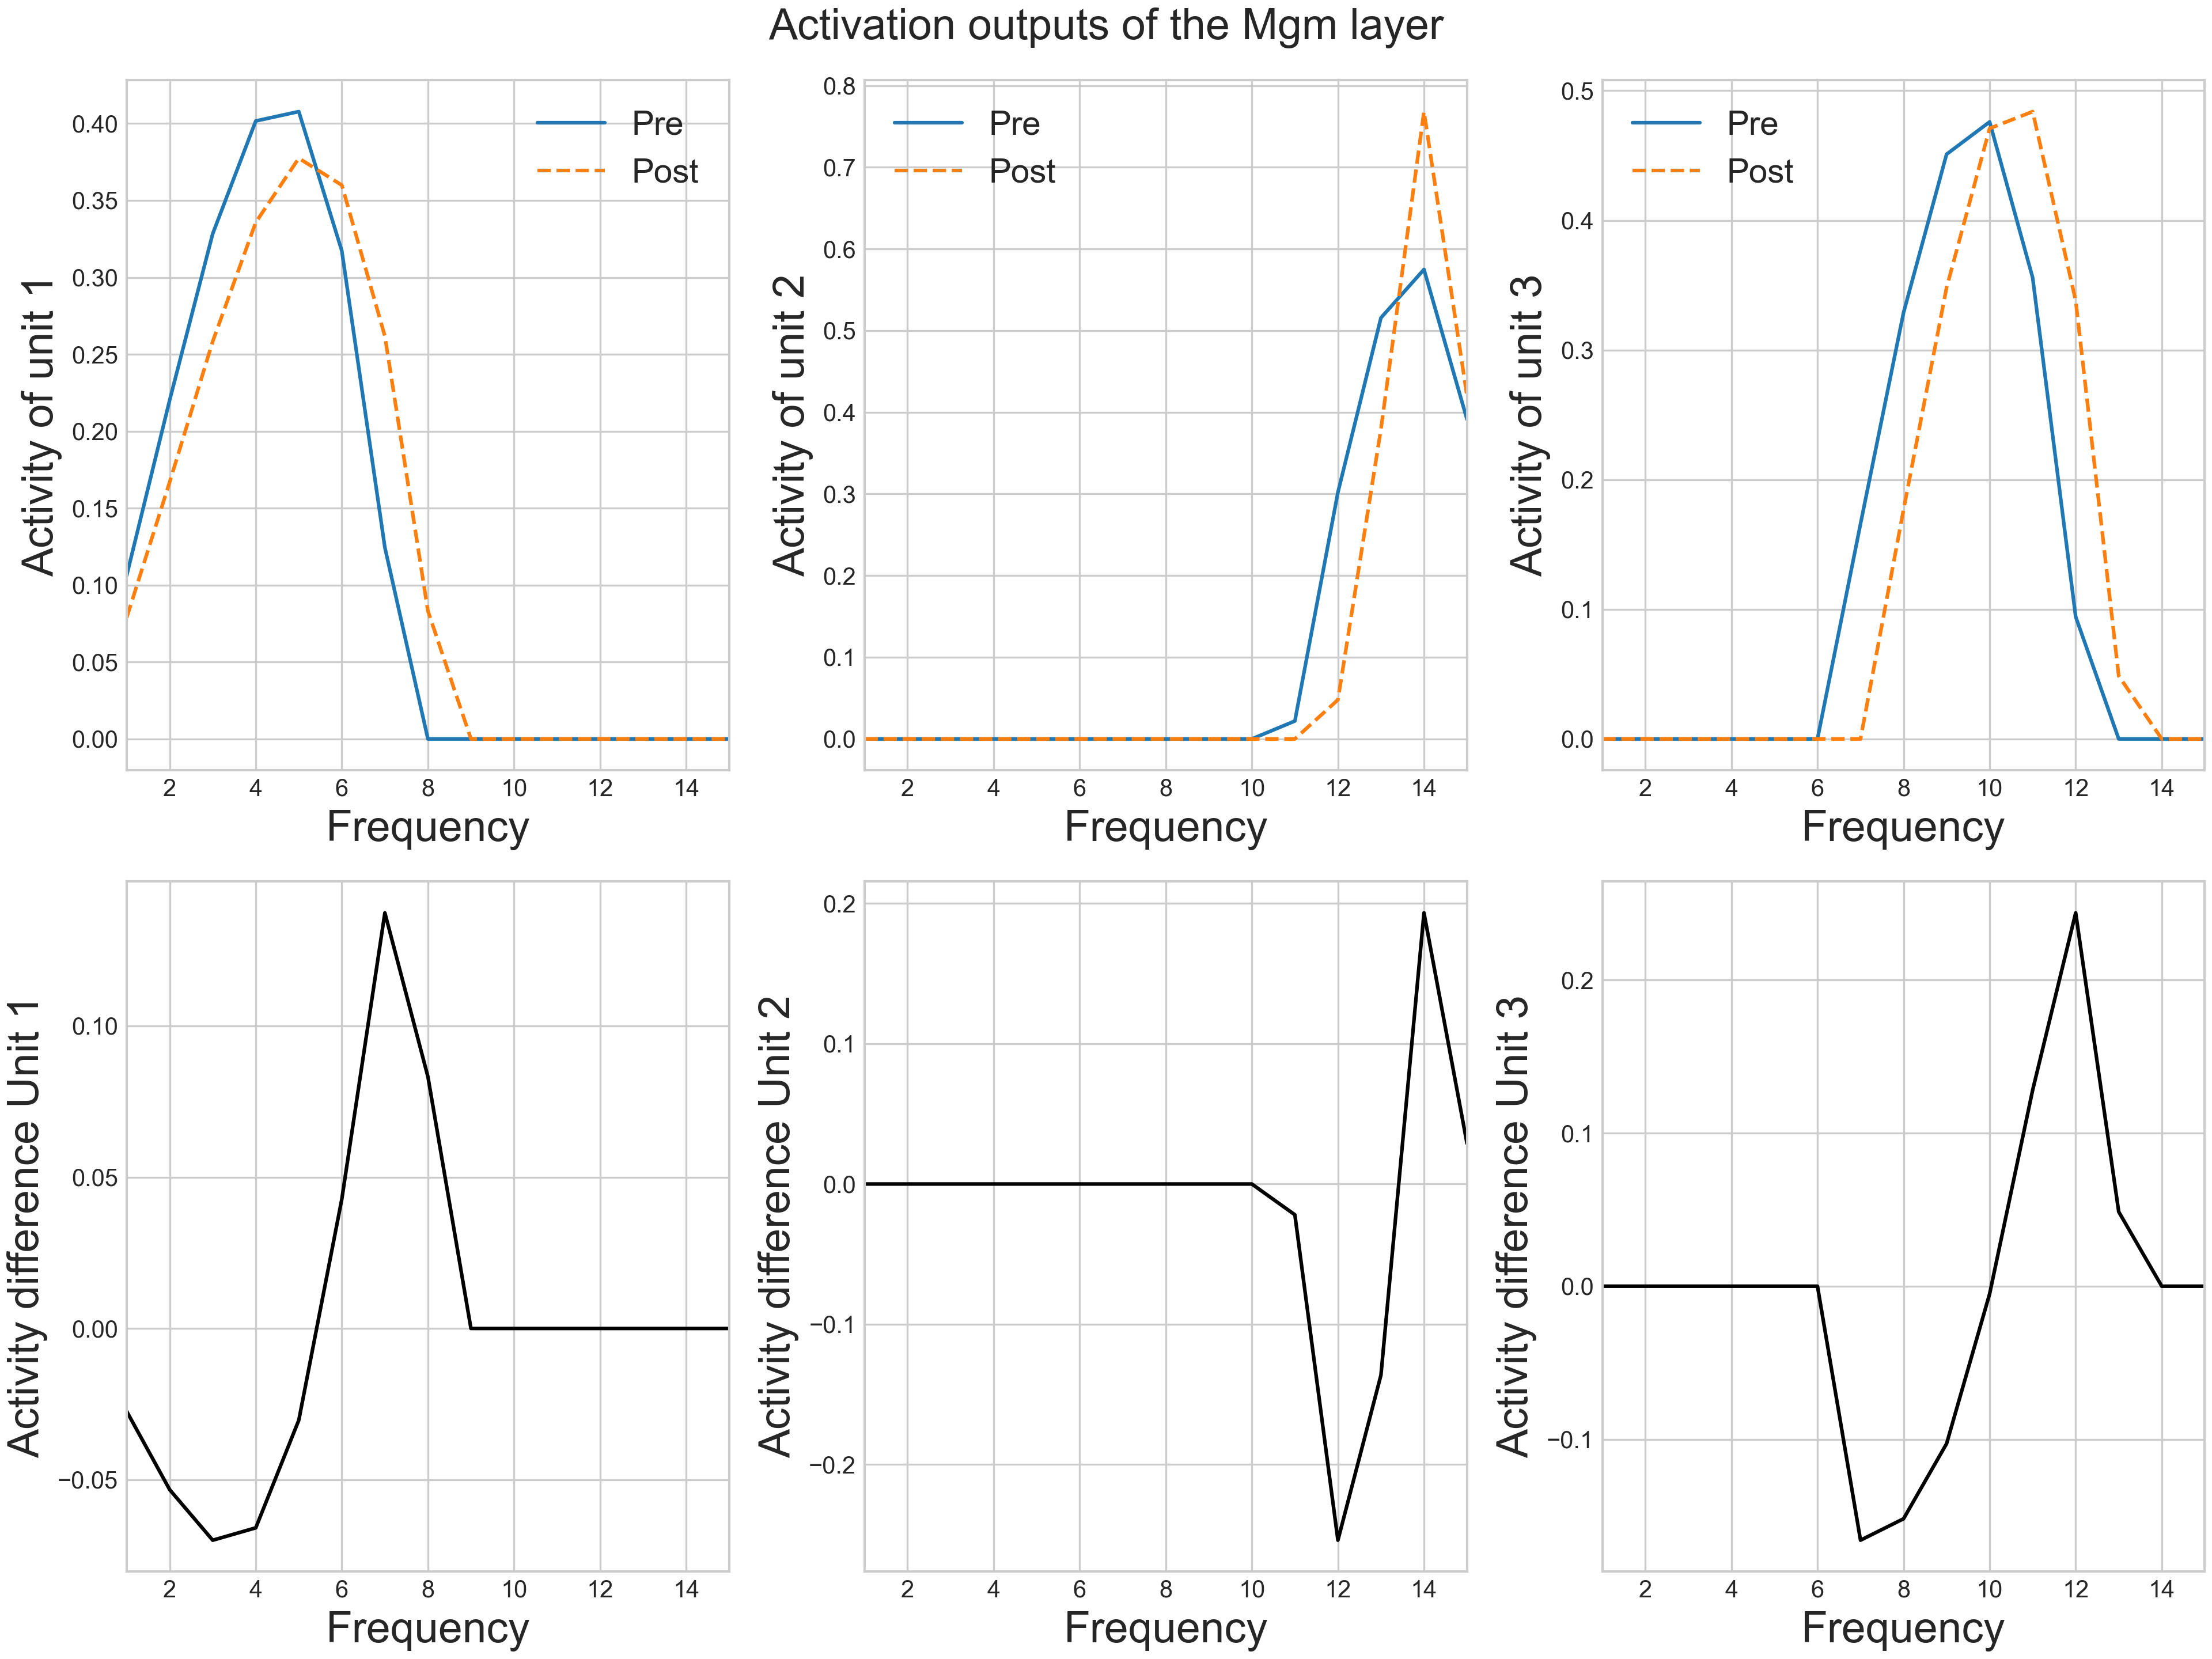
\includegraphics[width=\textwidth]{Figs/activation_mgm}
      \caption{\textit{This figure shows the activation of the neural units in the MGm layer at the end of the development phase (line labeled `\emph{Pre}') and after conditioning (labeled `\emph{Post}'). The difference in receptive fields are quite apparent, as is the increase in activity for the unit with a best frequency close to the frequency chosen as the CS (frequency $7$ in this case). The actual discrepancy in the activation of each unit before and after conditioning is made apparent by the set of graphs on the bottom line. As~\citet{Armony1995} remarked in the original paper, the receptive field of all units shift toward the CS, this is not a phenomenon limited to only a single unit.}}\label{fig:armony_act_mgm}
   \end{center}
\end{figure}

\begin{figure}[!htbp]
   \begin{center}
      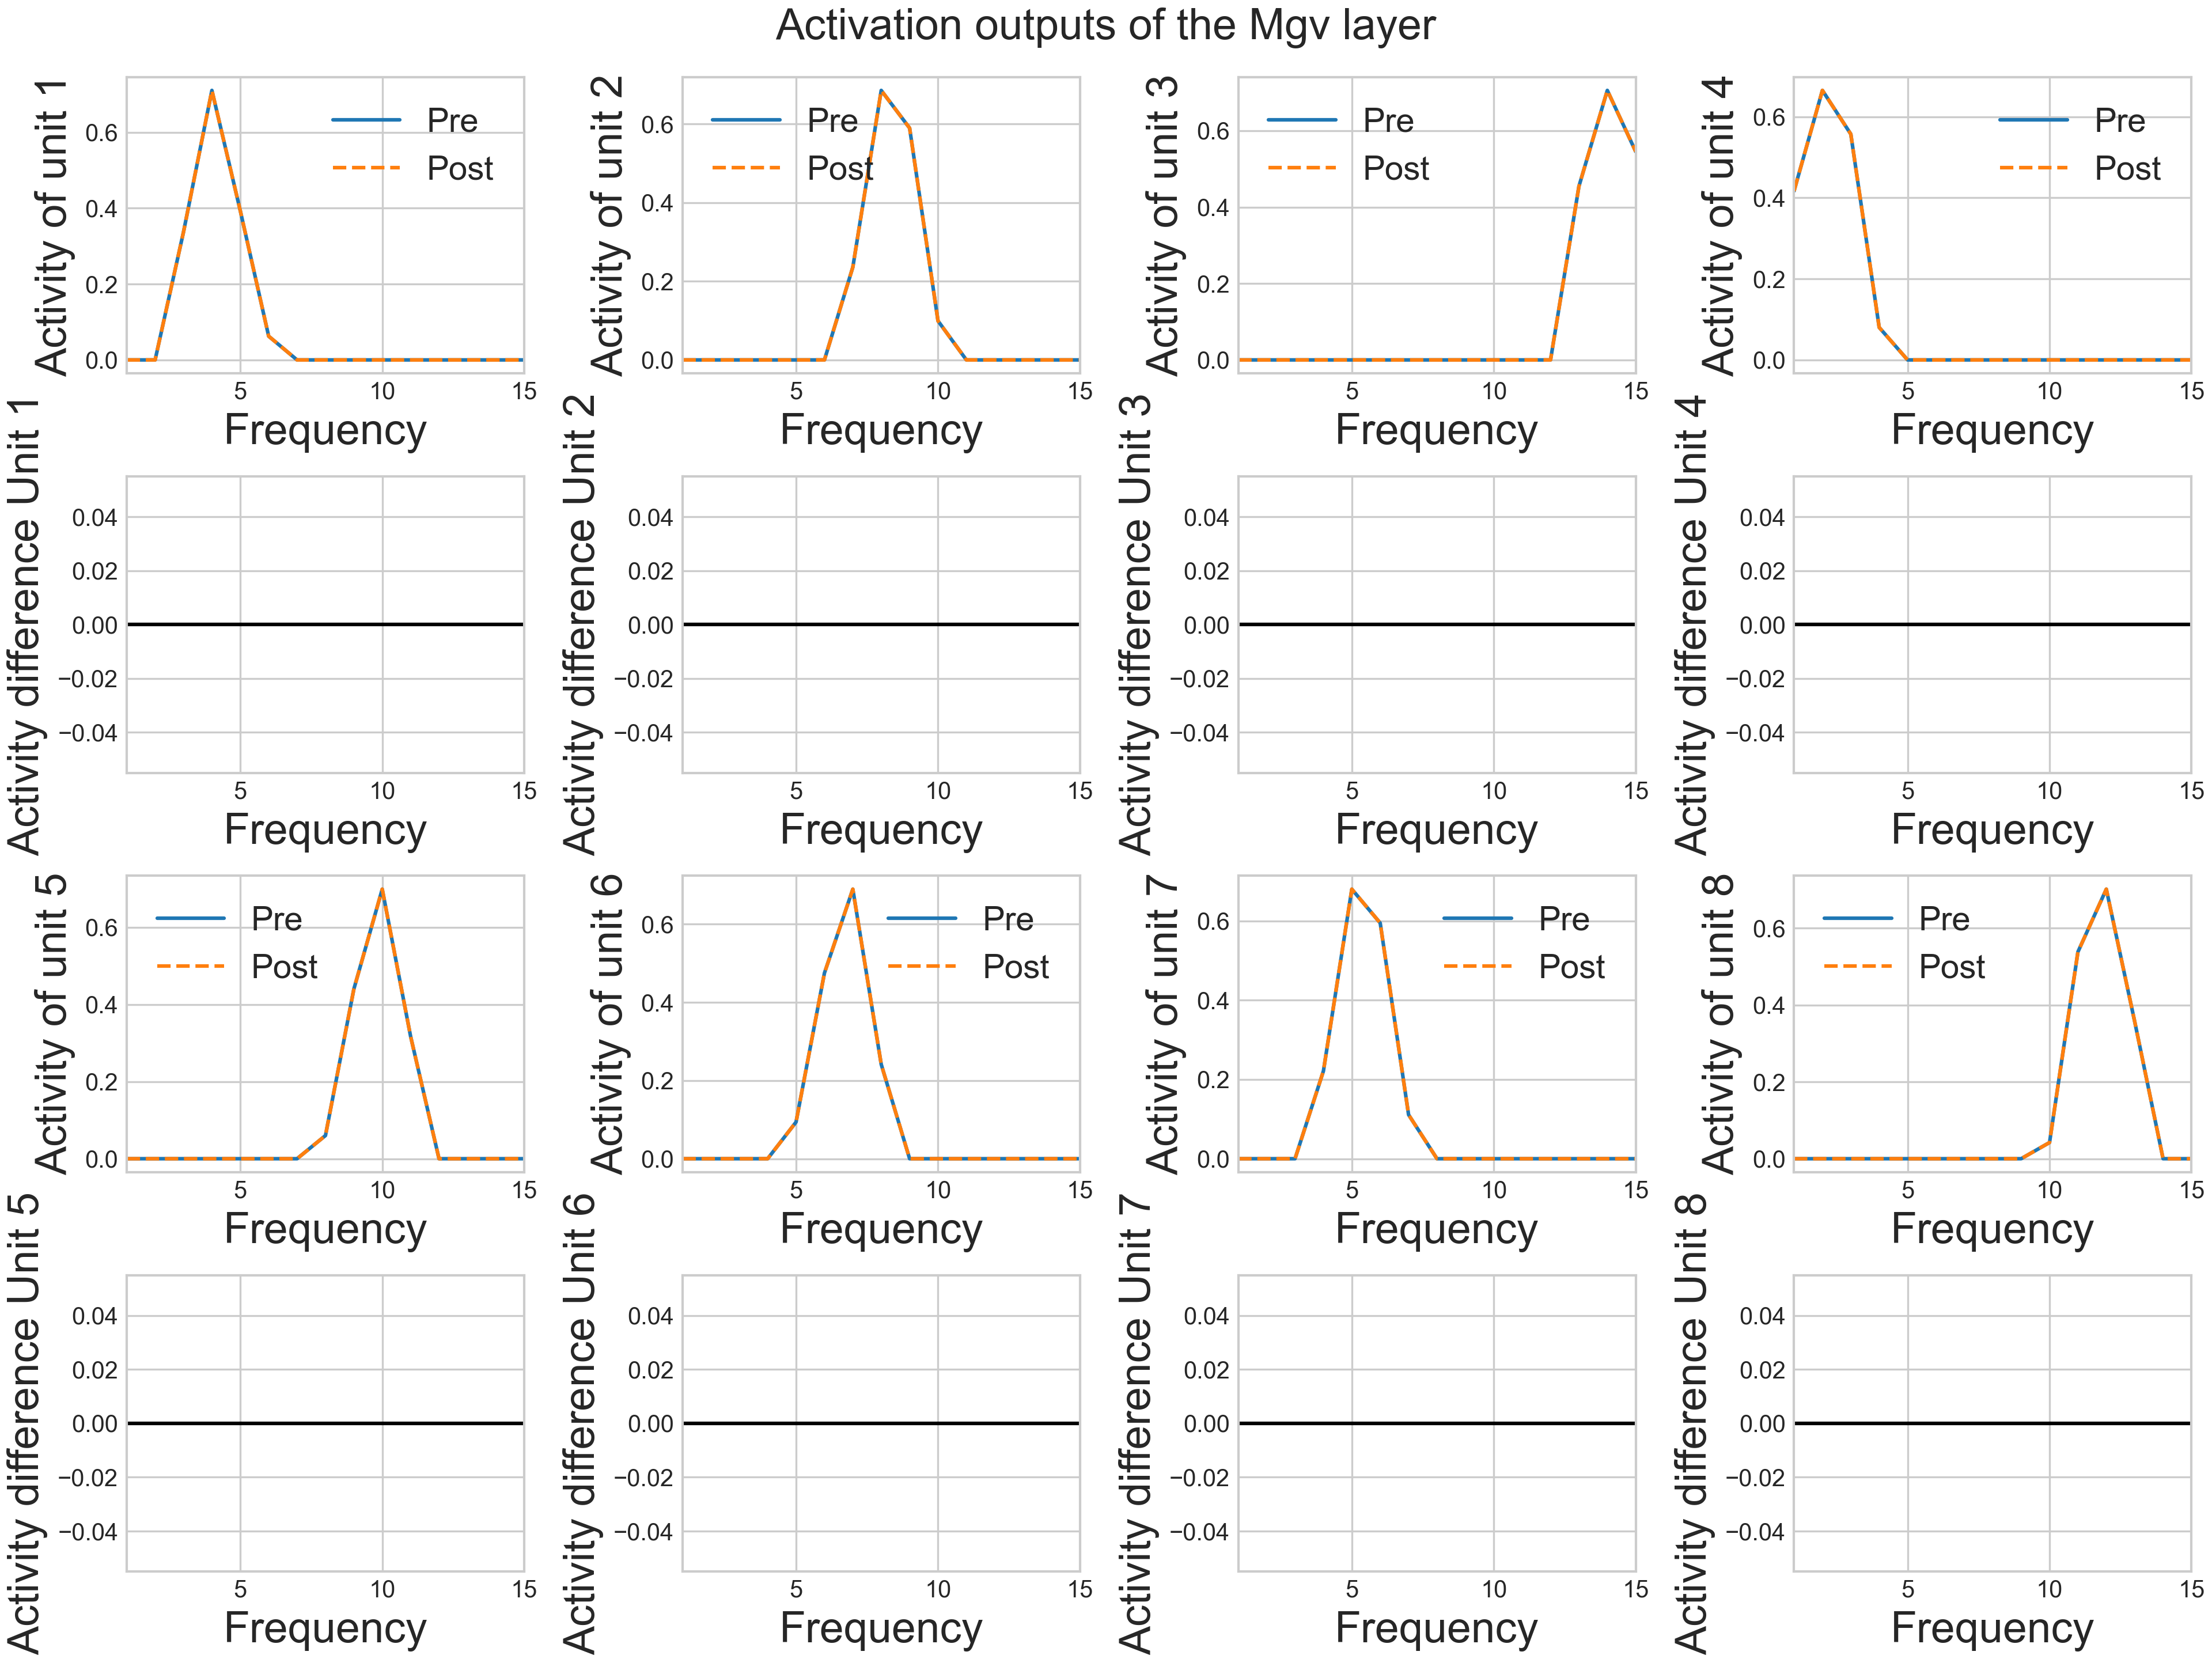
\includegraphics[width=\textwidth]{Figs/activation_mgv}
      \caption{\textit{This figure shows the activation of the neurons in the MGv layer pre- and post-conditioning. As mentioned by~\citet{Armony1995}, since the MGv does not receive any information about the nociceptive US the receptive fields of its neural units are not modified by the conditioning paradigm. This is made abundantly clear by the flat lines on the second and last row of this figure, which represent the difference in activity before and after conditioning for each unit.}}\label{fig:armony_act_mgv}
   \end{center}
\end{figure}

\begin{figure}[!htbp]
   \begin{center}
      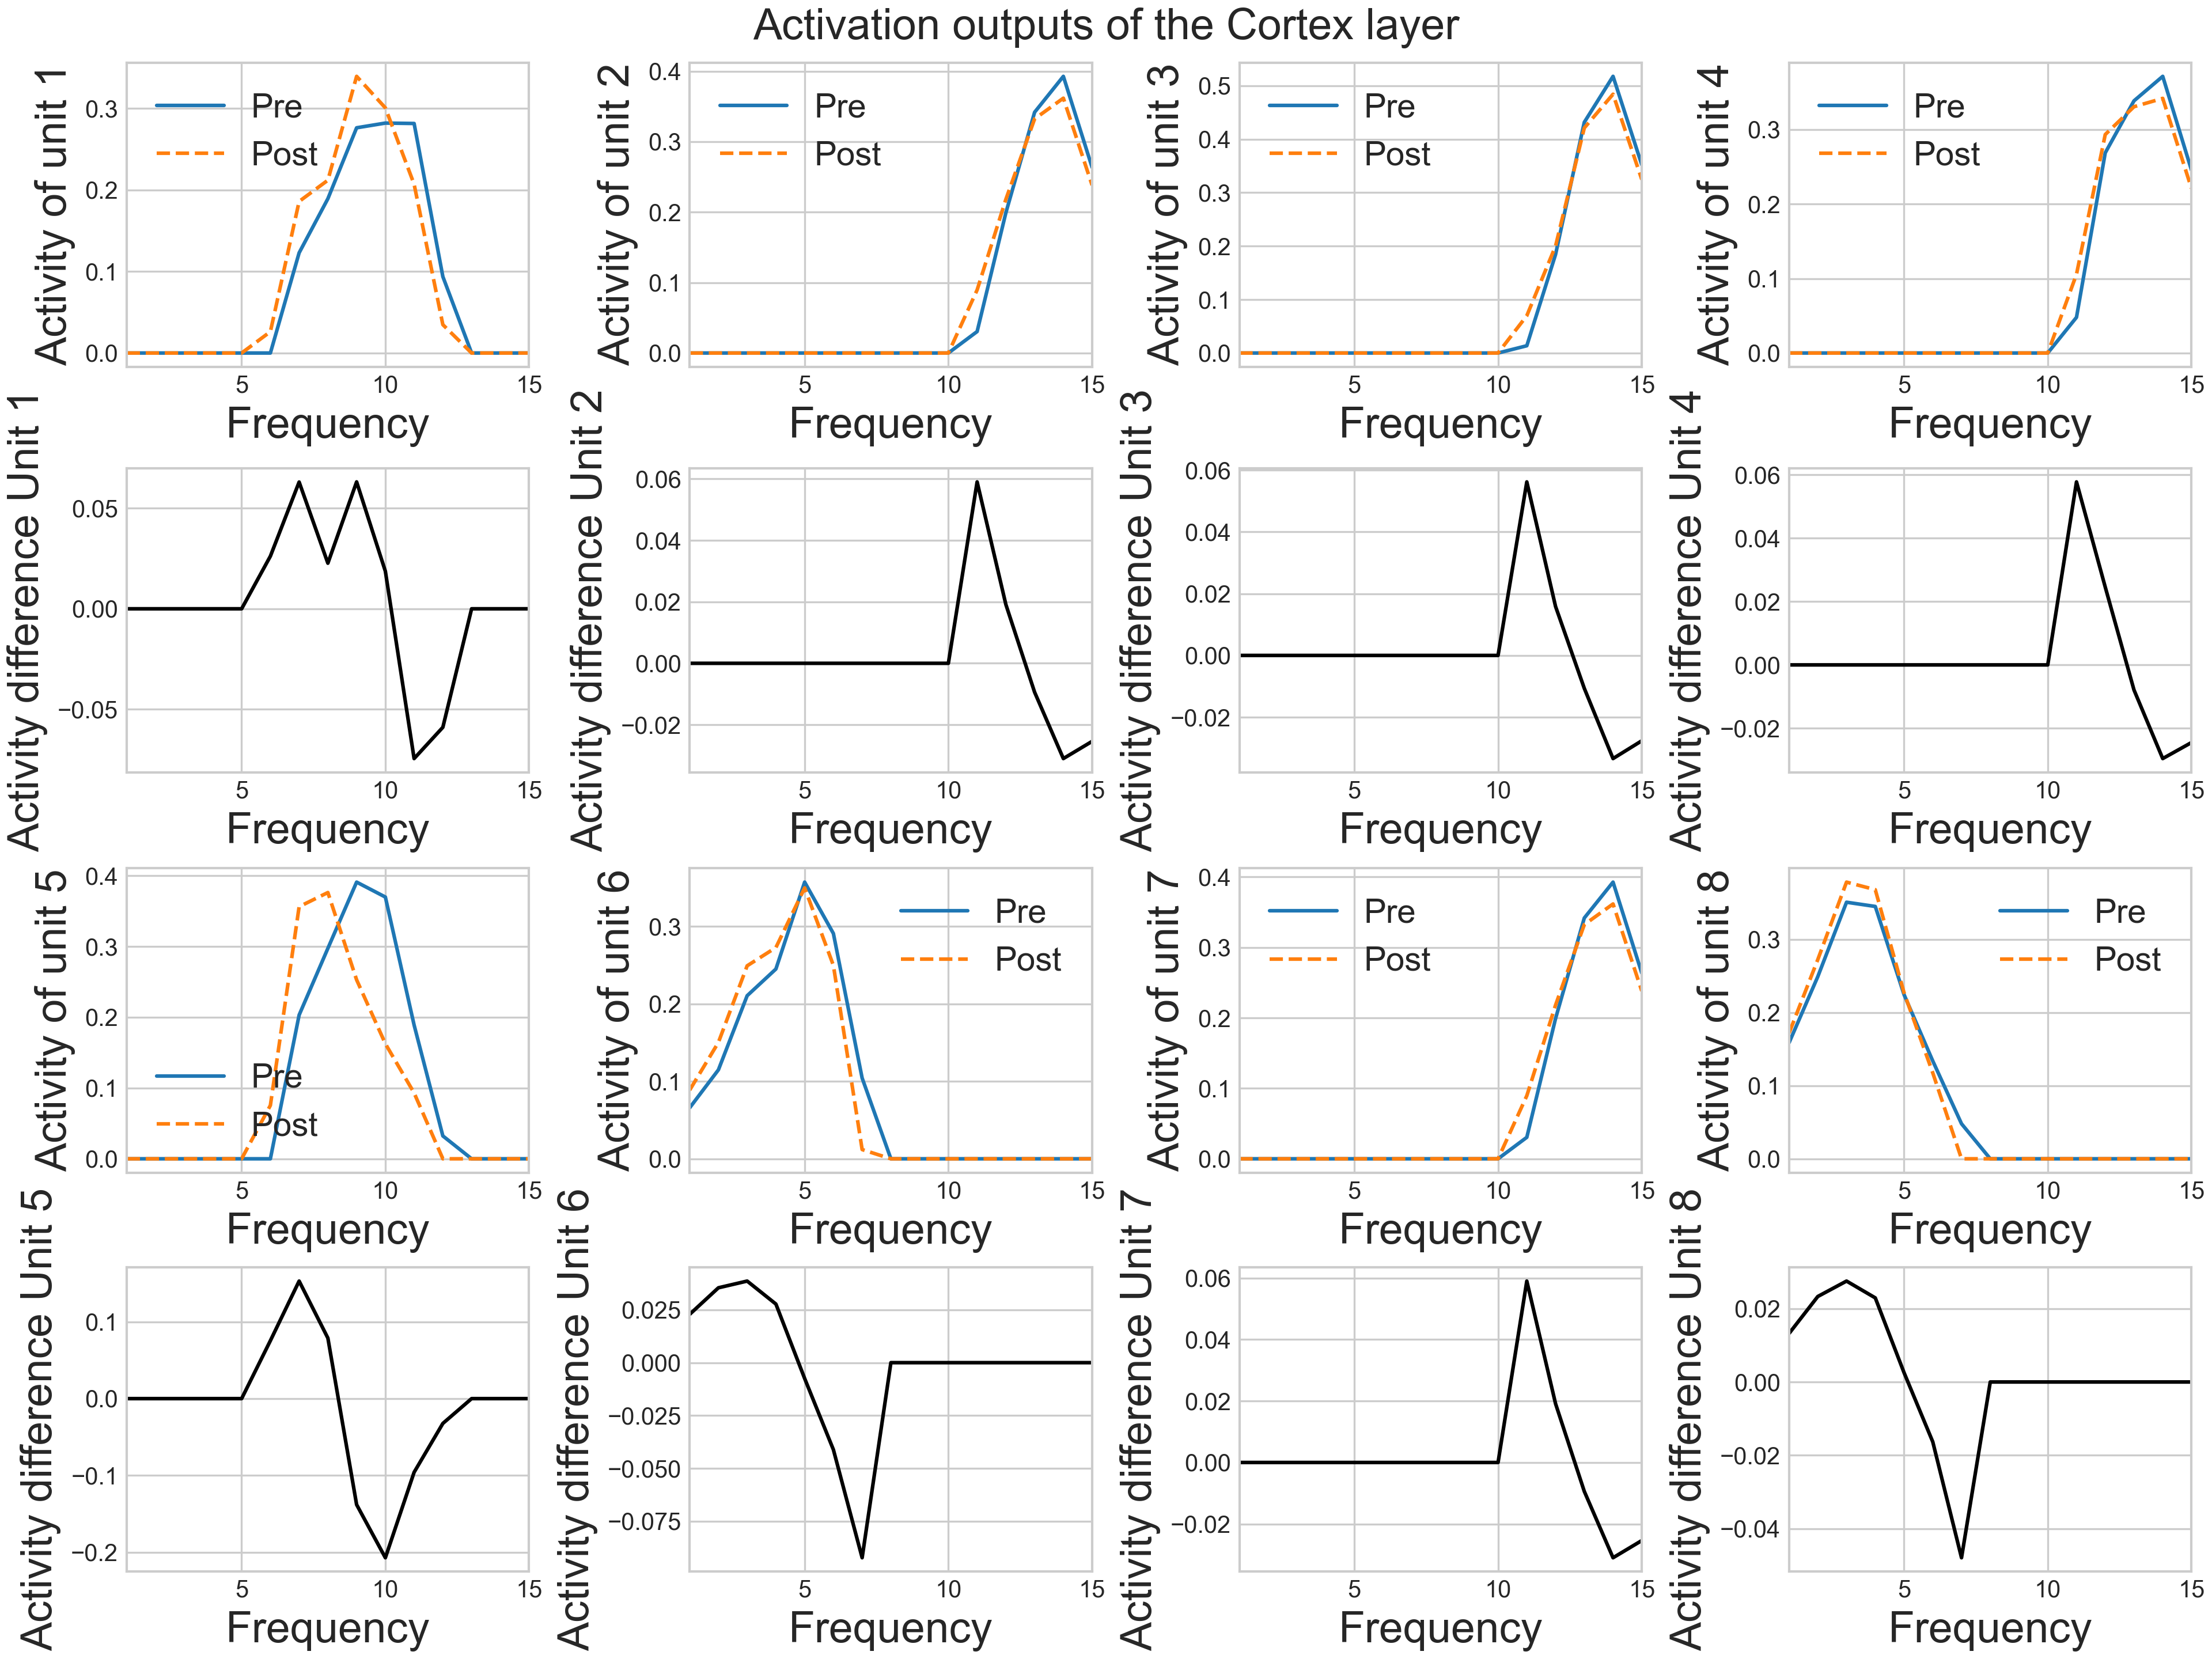
\includegraphics[width=\textwidth]{Figs/activation_cortex}
      \caption{\textit{This figure displays the activation of the neural units in the cortical layer before and after conditioning. Although, the auditory cortex does not receive any direct information about the nociceptive US, it does receive indirect data via the connections between the MGm and cortical layers. Hence, neurons inside the cortex also display a modification in their receptive field.}}\label{fig:armony_act_cortex}
   \end{center}
\end{figure}

\begin{figure}[!htbp]
   \begin{center}
      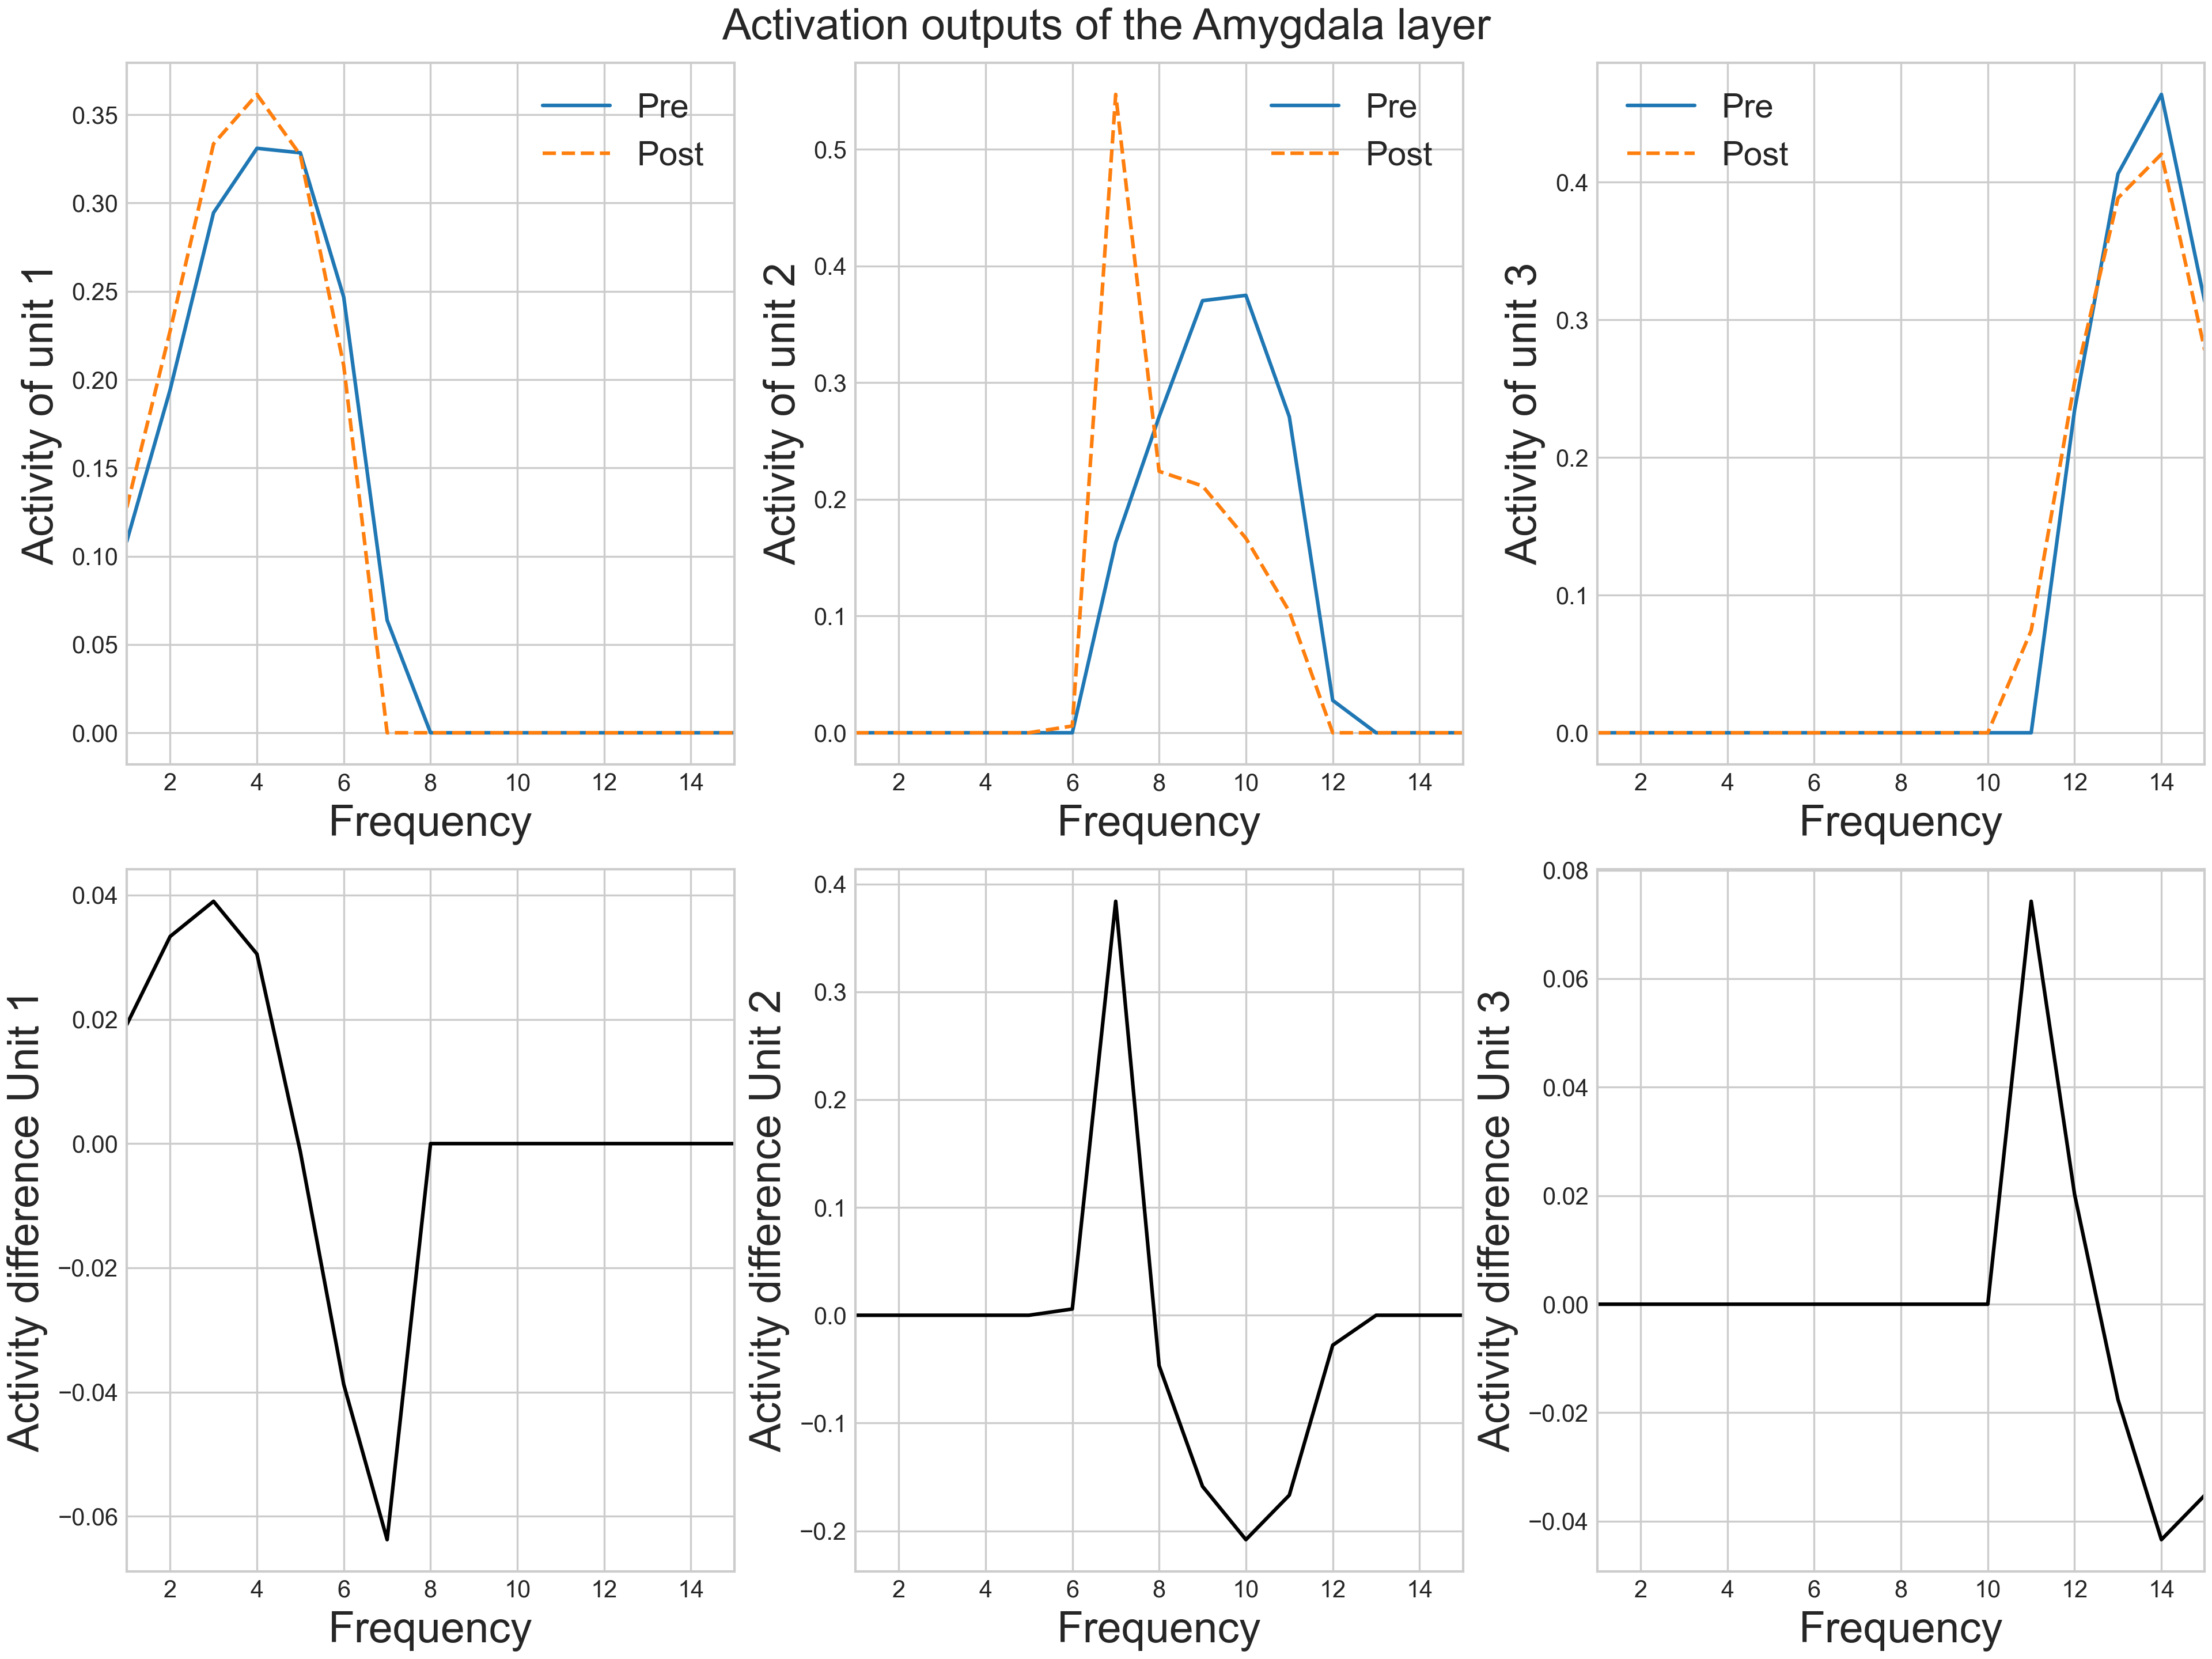
\includegraphics[width=\textwidth]{Figs/activation_amygdala}
      \caption{\textit{This figure depicts the activation of the neurons in the amygdala layer. According to~\citet{Ledoux1992} the amygdala is the target of two pathways. The first connecting directly the thalamus with the amygdala provides coarse information about incoming stimuli. The second pathway, going from the thalamus to the amygdala via the auditory cortex while slower than the first pathway, sends more fine-grained stimuli related data. Hence, the thalamo-cortico-amygdaloid path allows animals to be conditioned with tone of more specific frequencies, without reacting to tones with adjacent frequencies. In the model designed by~\citet{Armony1995} the amygdala, therefore, receives information directly from the nociceptive US, but also from the MGm and the cortical layers. As a result, the receptive fields of the different neural units are substantially modified after conditioning occurs.}}\label{fig:armony_act_amyg}
   \end{center}
\end{figure}

Finally the behavioral response, which is defined as the sum total of the amygdala's activities, produced a twofold increase in the network's response to the CS\@. Such a drastic change between pre- and post-conditioning output can be explained by the results presented in the previous paragraph. Indeed, given that units whose best frequency was close the CS prior to conditioning displayed a significant increase in their activity, it follows that the weighted sum of the activation values from those neurons would increase too. This aggregation of output activities also explains why the farther a frequency is from the CS the less intense the behavioral response is. As shown in Figure~\ref{fig:armony_behav_resp}, this results in a curve climbing as the tone comes closer to the CS, then reaching a peak for the CS, and falling back afterwards. It is further evidenced by the bottom plot of Figure~\ref{fig:armony_behav_resp}, which displays side-by-side the pre- and post-activity of the behavioral response at the CS frequency.

\begin{figure}[!htbp]
   \begin{center}
      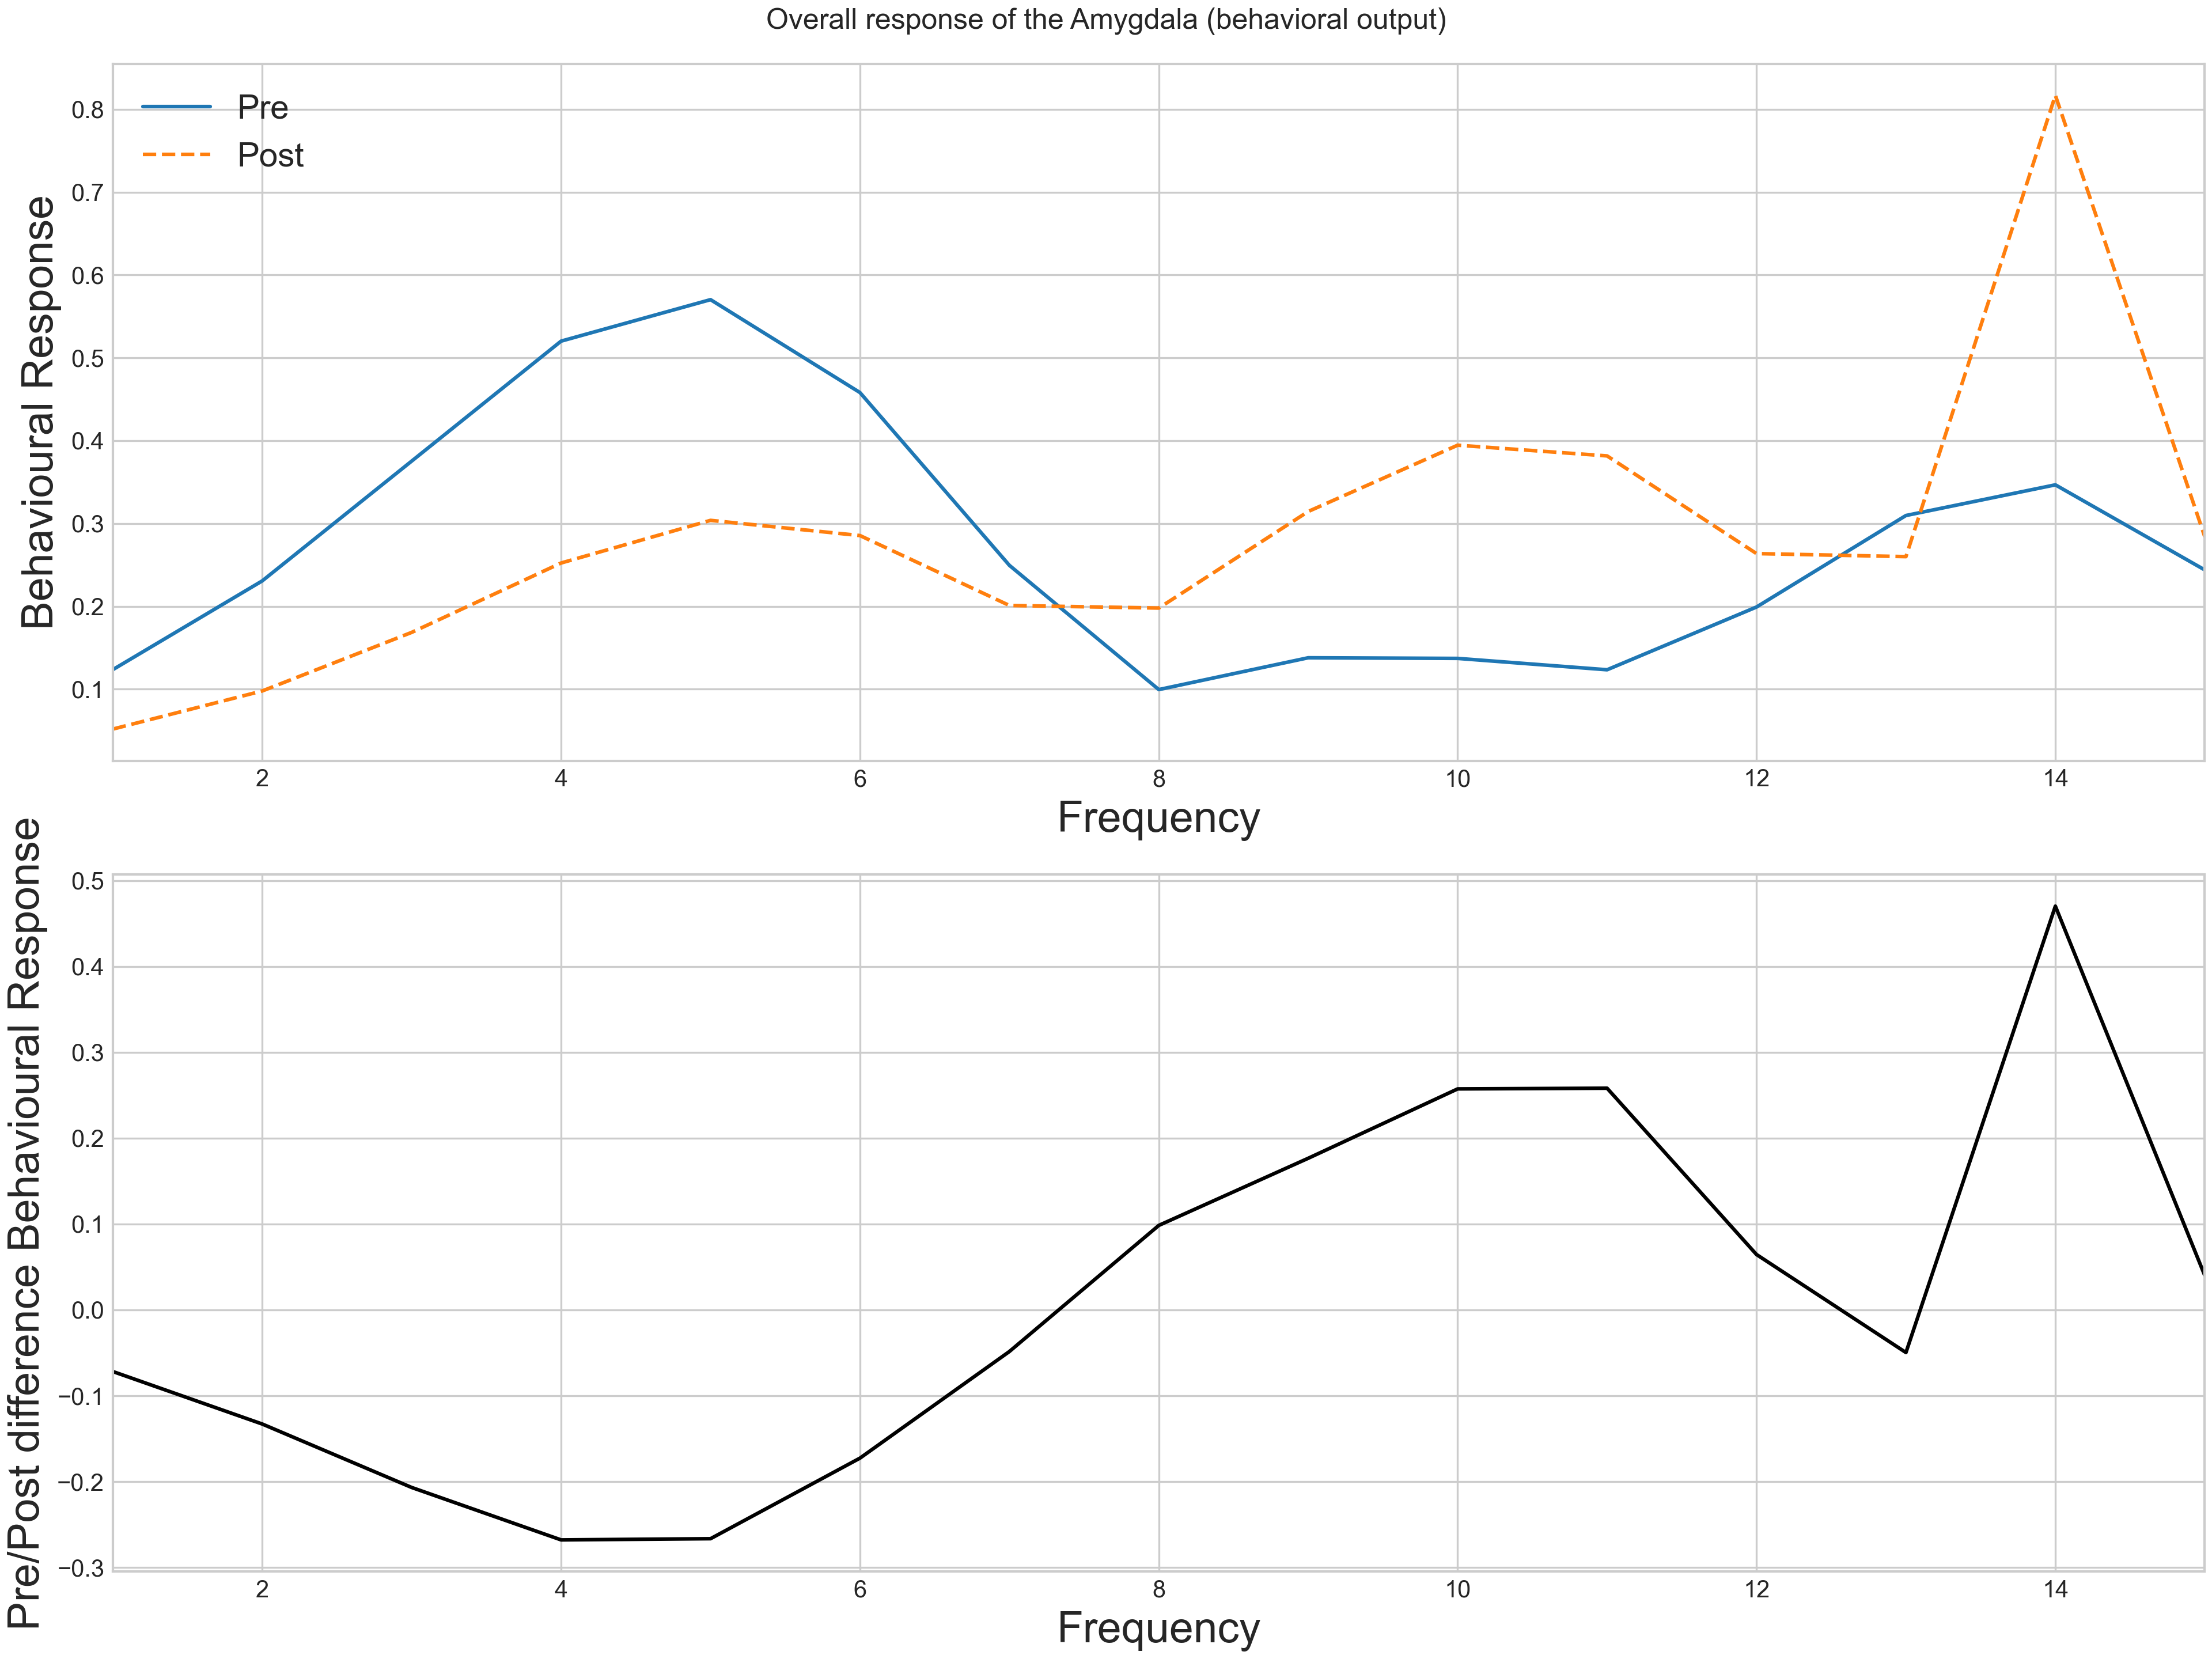
\includegraphics[width=\textwidth]{Figs/behavioral_response}
      \caption{\textit{This figure shows the evolution of the behavioral response against the different frequencies before and after conditioning. Since the behavioral response is defined as the total activity of the amygdala layer, and neurons in the amygdala see a drastic increase in activity around the CS frequency after conditioning, it follows that the behavioral response is at its maximum for the CS frequency. Activities for frequencies around the CS also see an increase in activity. However, the further a frequency is from the CS, the less it is impacted and can even decrease as a result of the shift in the receptive fields of the amygdala's neurons.}}\label{fig:armony_behav_resp}
   \end{center}
\end{figure}

\section{Conclusion}
The fear conditioning simulation re-created here based on the description from~\citet{Armony1995} seems to have yielded results similar to those published in the original paper. Due to the random initialization of the synaptic strengths in the development phase the match is not exact. However, the features necessary for drawing conclusions as to the validity of their principles are present in my observations as well.\\

In conclusion, the neural network was able to reproduce the overall behavior of the amygdala observed in fear conditioning experiments performed on animals. At the physiological level, the neural units did develop receptive fields that were subsequently altered via conditioning in a way similar to what was observed in single-cell recordings in animals (see~\citet{Armony1995} for graphs depicting those empirical results). As a consequence,~\citet{Armony1995} concluded that the principles that guided the design of the computational model were indeed correct. Meaning that the model of the dual pathways to the amygdala suggested by~\citet{Ledoux1992}, and~\citet{Romanski1992} can also be considered valid. More importantly though,~\citet{Armony1995} were able to show that:
\begin{quotation}
   ``\textit{\dots a neuroanatomically constrained network, together with a biologically plausible learning algorithm, can capture important aspects of the behavioral and physiological consequences of fear conditioning. The model offers a complementary approach to experimental studies for examining issues pertaining to the acquisition and expression of fear learning in the brain.}'' ---~\citet{Armony1995}
\end{quotation}
Furthermore, results pertaining to the simulation of a lesion study~\supercite{Armony1997,Armony1997a}, proved the model capable of predicting the effects of severing the connections between different parts of the network. Thus, adding their voices to the mounting evidence that computational models should be an essential tool in the belt of any neuroscientist.
